\section{Bartłomiej Wolny}
A basic equation known to all of us, even beavers (Figure 1):

\begin{equation}
i \hbar \frac{\partial}{\partial t}\Psi(\mathbf{r},t) = \hat H \Psi(\mathbf{r},t)
\end{equation}

\begin{figure}[H]
    \centering
    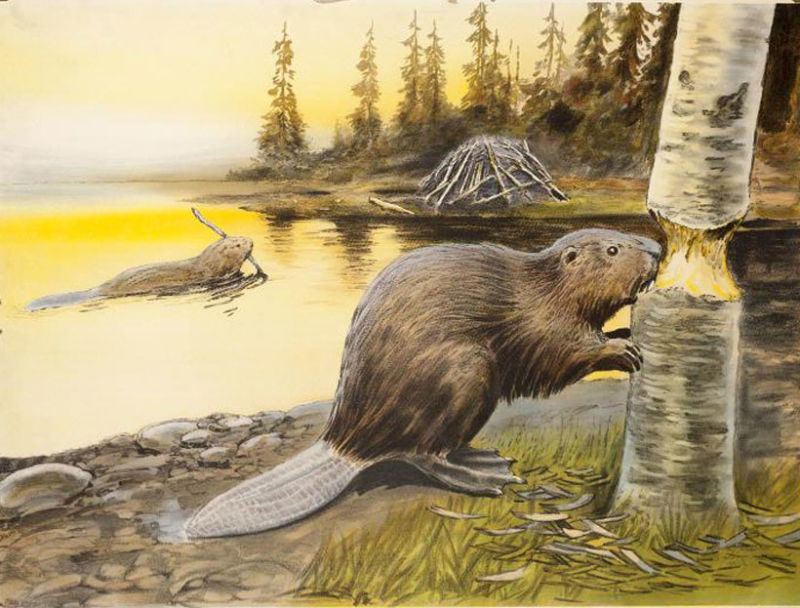
\includegraphics[width=.55\textwidth]{pictures/Beaver-hero.jpg}
    \caption{Beavers may have known this equation before us. This is a photo of one of them chopping a tree down with its teeth.}
    \label{fig:beaver-image}
\end{figure}

\begin{itemize}
    \item Test of dots
    \item Second dot
    \item Third one
\end{itemize}


\begin{table}[H]
\centering
\begin{tabular}{|c|c|c|}
\hline
\textbf{Age} & \textbf{Weight (kg)} & \textbf{Tail Length (cm)} \\
\hline
1 & 6 & 24 \\
2 & 8 & 28 \\
3 & 10 & 32 \\
4 & 12 & 36 \\
5 & 14 & 40 \\
\hline
\end{tabular}
\caption{Beaver Data}
\end{table}

\textbf{Beavers, celebrated as nature's master architects, wield their construction prowess to sculpt intricate dams and lodges, not only providing shelter for their own kin but also orchestrating an ecological symphony that nurtures wetland ecosystems and fosters biodiversity.} Their remarkable role as builders and environmental stewards underscores the profound interplay between species and their habitats, exemplifying the intricate tapestry of life within our natural world.
